\documentclass{article}
\usepackage[utf8]{inputenc}
\usepackage{tikz}
\usetikzlibrary{shapes.geometric,arrows}

\tikzstyle{startstop} = [rectangle,rounded corners, minimum width=3cm,minimum height=1cm,text centered, draw=black,fill=red!30]
\tikzstyle{io} = [trapezium, trapezium left angle = 70,trapezium right angle=110,minimum width=3cm,minimum height=1cm,text centered,draw=black,fill=blue!30]
\tikzstyle{process} = [rectangle,minimum width=5cm,minimum height=1cm, text centered, text width =6cm,draw=black,fill=orange!30]
\tikzstyle{decision} =[diamond,minimum width=4cm,minimum height=1cm, text centered,draw=black,fill=green!30]
\tikzstyle{arrow} = [thick,->,>=stealth]

\begin{document}

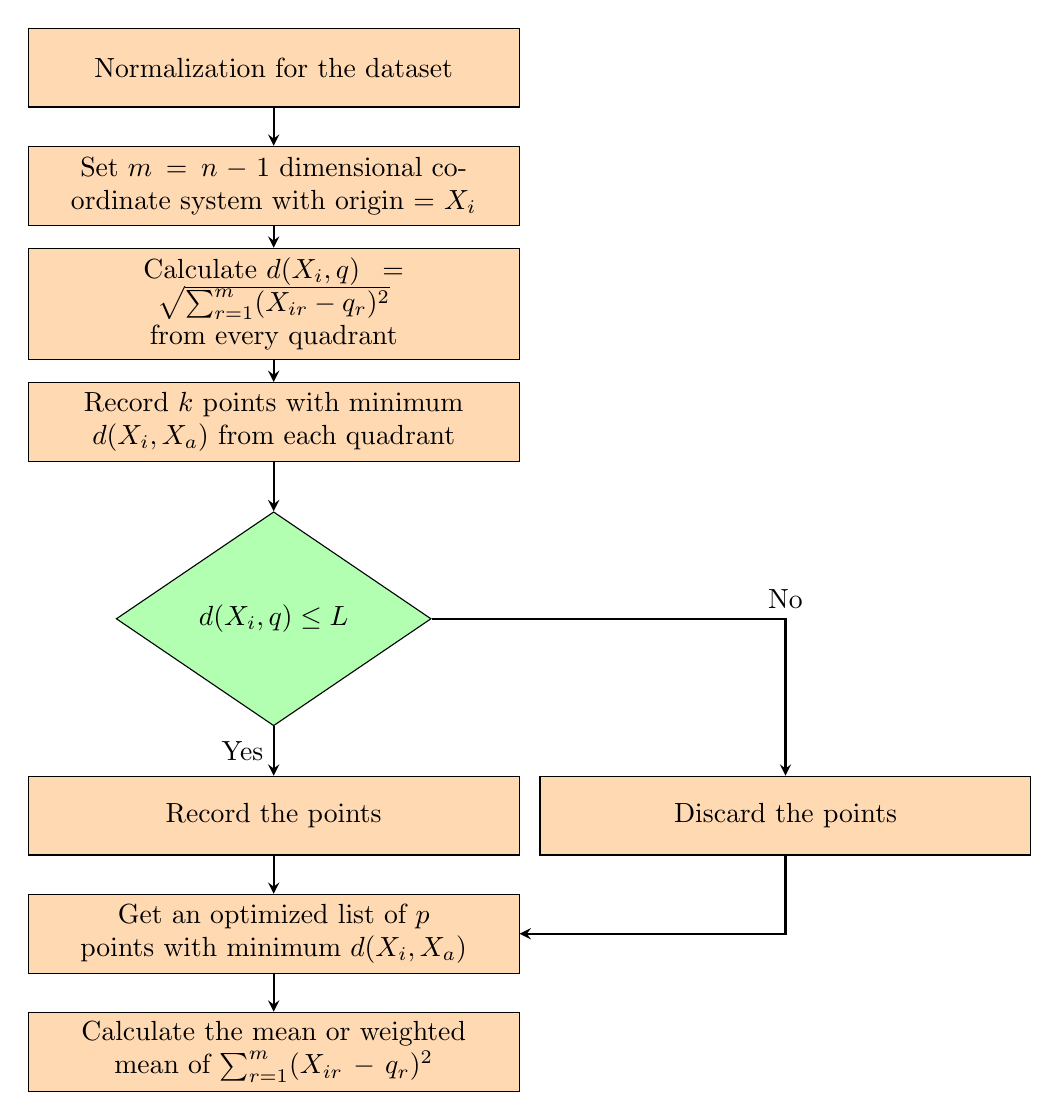
\begin{tikzpicture}[node distance = 1.5cm]

% \node (start) [startstop] {Start};
% \node (in1) [io] {Input};
\node(pro) [process] {Normalization for the dataset};
% \node(pro1) [process, below of=pro] {Multiple linear regression $X_{i} = f(X_{1}, \dots, X_{i-1}, X_{i+1}, \dots, X_{n})$, select $m$ instrumental variables for $X_{i}$};
% \node(dec1) [decision, below of=pro1, yshift=-1cm] {$m \geq 0$};
% \node(pro2a) [process, below of=dec1, yshift = -1cm] {Set $m$ dimensional coordinate system with origin = missing $X_{i}$};
\node(pro2) [process, below of =pro] {Set $m=n-1$ dimensional coordinate system with origin = $X_{i}$};
\node(pro3) [process, below of=pro2] {Calculate $d(X_{i}, q) = \sqrt{\sum_{r=1}^{m} (X_{ir}-q_{r})^2}$ from every quadrant};
\node(pro4) [process, below of=pro3] {Record $k$ points with minimum $d(X_{i}, X_{a})$ from each quadrant};
\node(dec2) [decision, below of=pro4, yshift=-1cm] {$d(X_{i}, q)\leq L$};
\node(pro5) [process, below of=dec2, yshift=-1cm] {Record the points}; 
\node(pro6) [process, right of=pro5, xshift=5cm] {Discard the points}; 
\node(pro7) [process, below of=pro5] {Get an optimized list of $p$ points with minimum $d(X_{i}, X_{a})$};
\node(pro8) [process, below of=pro7] {Calculate the mean or weighted mean of $\sum_{r=1}^{m} (X_{ir}-q_{r})^2$};



\draw [arrow] (pro) -- (pro2);
% \draw [arrow] (dec1) -- node[anchor=east]{Yes}(pro2a);
% \draw [arrow] (dec1) -| node[anchor=south]{No}(pro2b);
\draw [arrow] (pro2) -- (pro3);
% \draw [arrow] (pro2b) |- (pro3);
\draw [arrow] (pro3) -- (pro4);
\draw [arrow] (pro4) -- (dec2);
\draw [arrow] (dec2) -- node[anchor=east]{Yes}(pro5);
\draw [arrow] (dec2) -| node[anchor=south]{No}(pro6);
\draw [arrow] (pro5) -- (pro7);
\draw [arrow] (pro6) |- (pro7);
\draw [arrow] (pro7) -- (pro8);


\end{tikzpicture}

\end{document}


